% Drawing 104/01-3 -- folder 104, batch 01, archive page 3 (PDF page 4).
% Transcription: moitié droite du feuillet, six figures : en haut, un prisme oblique à faces hachurées posé sur un quadrillage de quatre colonnes et trois rangées ; un segment aux extrémités marquées ; un rectangle ouvert à droite, ses côtés haut et bas épaissis ; un carré aux quatre sommets marqués ; un cylindre dont la base est une amande hachurée à deux sommets ; plus bas, un carré divisé en quatre.
% Kind: prism on a grid, segment, open rectangle, square, cylinder with an almond base, square cut in four. Method 2 (schematic redraw from the facsimile). Status: partial.
% Notes: Top: the grid (four columns, three rows) with its heavy oblique hatching strokes, one per column, and above it the slab drawn in perspective: five oblique edges rising to the right from the top of the grid, the top edge, the right-hand vertical and the oblique edge closing the right side. Then the segment with its two end marks; the rectangle open at the right (top and bottom sides heavy); the square with its four marked corners (left and top sides heavy); the cylinder: top rim as two arcs, two sides, and the base as an almond between two marked points, hatched with vertical strokes; and, lower on the sheet, the square cut in four. Left out: the formulas between the figures and the typescript showing through. Still differs: the prism is a crowded perspective sketch; its strokes are regularised and the inner rectangle drawn on its top face is omitted; the note of the transcription counts four figures (prism, square, cylinder, square cut in four): the segment and the open rectangle are added here. Overlaid on the 400 dpi colour facsimile on 2026-11-12 (Opus 5.5) and corrected: the square cut in four at the foot was drawn 2 to 3 mm too low at its top and middle lines; redrawn from the page: its top line stops short of the upper right corner (the right side starts lower), the middle line stands at mid-height, the dividing vertical runs a little past the top and bottom. The other figures lie on the page within 1 to 2 mm; the prism stays as described above. Redrawn 2026-11-12 (issue 128): to check again. 2026-11-13, Claude Opus 5.5, overlay check (issue 147): laid over the scan rendered at 350 dpi in colour; not compiled (no TeX engine in the session), the TikZ was rasterised by a script; nothing changed. The segment, the open rectangle, the square with its four marked corners, the cylinder and the square cut in four lie on their ink within about 1 to 2 units. Kept partial for the prism: its base grid is drawn as a regular rectangular grid where his is a skewed parallelogram with lines running past it, its hatching strokes and receding edges are regularised (1 to 3 units off), and the inner rectangle of its top face is omitted.
% Coordinates: 1 unit = 1 mm = 1/100 of the crop width (bbox in page fractions: [0.55, 0.075, 0.88, 0.47]).
% Redrawn by Claude (claude-fable-5-2), issue #128, 2026-11-12; not checked by a human; not compiled (no TeX in the session).
% Corrected by Claude (claude-opus-5-5) 2026-11-12 (issue #128): overlaid on the 400 dpi colour facsimile and corrected from it. Not compiled. Status: partial.
% Rights: reproduces part of the work -- behind RENDER_TRANSCRIPTS, never published by itself.
\documentclass[tikz,border=3pt]{standalone}
\usepackage{amsmath,amssymb}
\usetikzlibrary{patterns,arrows.meta}
\tikzset{pencil/.style={black!45}, struck/.style={black!35}, mpt/.style={circle,draw,inner sep=1.3pt}, pt/.style={circle,fill,inner sep=0.9pt}, opt/.style={circle,draw,fill=white,inner sep=1.1pt}}
\begin{document}
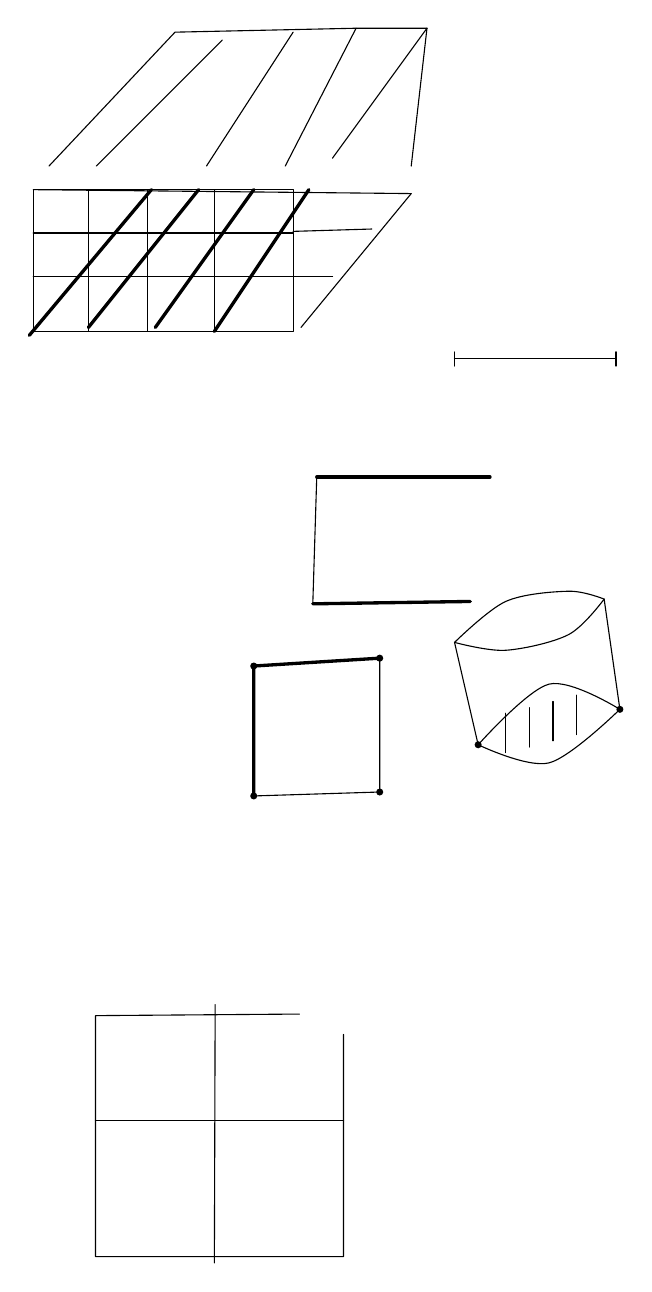
\begin{tikzpicture}[x=1mm,y=1mm,line cap=round,line join=round,font=\scriptsize]
\draw (12,-30) -- (45,-30) -- (45,-48) -- (12,-48) -- cycle;
\draw (19,-30) -- (19,-48);
\draw (26.5,-30) -- (26.5,-48);
\draw (35,-30) -- (35,-48);
\draw (12,-35.5) -- (45,-35.5);
\draw (12,-41) -- (45,-41);
\draw (12,-30) -- (60,-30.5);
\draw (45,-35.3) -- (55,-35);
\draw (45,-41) -- (50,-41);
\draw[very thick] (11.5,-48.5) -- (27,-30);
\draw[very thick] (19,-47.5) -- (33,-30);
\draw[very thick] (27.5,-47.5) -- (40,-30);
\draw[very thick] (35,-48) -- (47,-30);
\draw (14,-27) -- (30,-10);
\draw (20,-27) -- (36,-11);
\draw (34,-27) -- (45,-10);
\draw (44,-27) -- (53,-9.5);
\draw (50,-26) -- (62,-9.5);
\draw (30,-10) -- (53,-9.5) -- (62,-9.5);
\draw (62,-9.5) -- (60,-27);
\draw (60,-30.5) -- (46,-47.5);
\draw (65.5,-51.5) -- (86,-51.5);
\draw (65.5,-50.6) -- (65.5,-52.4);
\draw (86,-50.6) -- (86,-52.4);
\draw[very thick] (70,-66.5) -- (48,-66.5);
\draw (48,-66.5) -- (47.5,-82.6);
\draw[very thick] (47.5,-82.6) -- (67.5,-82.3);
\draw[very thick] (40,-107) -- (40,-90.5) -- (56,-89.5);
\draw (56,-89.5) -- (56,-106.5) -- (40,-107);
\node[pt] at (40,-90.5) {};
\node[pt] at (56,-89.5) {};
\node[pt] at (56,-106.5) {};
\node[pt] at (40,-107) {};
\draw plot[smooth, tension=0.55] coordinates {(65.5,-87.5) (72,-82.3) (80,-81) (84.5,-82)};
\draw plot[smooth, tension=0.55] coordinates {(65.5,-87.5) (72,-88.5) (80,-86.5) (84.5,-82)};
\draw (65.5,-87.5) -- (68.5,-100.5);
\draw (84.5,-82) -- (86.5,-96);
\draw plot[smooth, tension=0.55] coordinates {(68.5,-100.5) (77.5,-92.8) (86.5,-96)};
\draw plot[smooth, tension=0.55] coordinates {(68.5,-100.5) (77.5,-102.8) (86.5,-96)};
\node[pt] at (68.5,-100.5) {};
\node[pt] at (86.5,-96) {};
\draw (72,-96.5) -- (72,-101.5);
\draw (75,-95.8) -- (75,-100.8);
\draw (78,-95) -- (78,-100);
\draw (81,-94.2) -- (81,-99.2);
\draw (45.8,-134.7) -- (19.9,-134.9) -- (19.9,-165.5) -- (51.4,-165.5) -- (51.4,-137.3);
\draw (35.1,-133.5) -- (35,-166.3);
\draw (19.9,-148.2) -- (51.4,-148.2);
\end{tikzpicture}
\end{document}
